\part{Towards Highly Miniaturized LED Power Systems }
\label{ch:twrd_HMLED}

\chapter[LEDification]{LEDification means Power System Integration}


The light bulb was one of the most relevant inventions form our past history.  Electrical lighting was definitely a revolution in the early 19$^{th}$ century society; for the first time in the history people had a clear, reliable and safe source of artificial light that was easy to distribute and control.
The apparition  of the electrical light bulb was also, with no doubt, the trigger for the commercialization of electric power and the deployment of the first power distribution networks. The impact was to such degree that it settled two of capital sectors from the present industry, the lighting and the electric power distribution, with  world recognized companies such as Philips, General Electric or Osram.  Actually, both sectors have been so close related that even often we use the word \emph{light} when we actually are meaning \emph{electricity}. In resume, a single invention changed our society for ever, bringing light and electricity to our homes.

\begin{figure}[!h]
\centering
\includegraphics{./0_intro/img/1900-philips3.jpg}
\caption{Philips commercial comparing what was before \emph{Vroeger} an oil lamp and was \emph{Today the} incandescent light bulb}
\label{fig:incandescent_light_blub}
\end{figure}


From the initial invention of the first incandescent light bulb,  bulbs have just been illuminating our daily lives without having  any \emph{enlightening} relevance or sense of innovation. Despite our impression,  important research has continuously been done to improve the worst characteristic of the incandescent light bulb, the efficacy. Incandescent light bulbs are extremely inefficient generating light, with a luminous efficacy between $12.6 lm/W$ for a tungsten incandescent bulb, and  up to $24 lm/W$ for a quartz halogen bulb (see Table~\ref{tab:lighting_tech}). In a more comprehensive way, we can say that in general incandescent lights convert at least 95\% of the supplied power in heat and just, at most 5\% in light. Knowing that lighting represents 17\% of world energy consumption, we can account that 15\% of the world consumed power is transformed in to heat and only a 1.7\% is transformed in real light \footnote{Estimated values for the year 2008}. Therefore these figures illustrate  the motivation and necessity of improving the efficacy/efficency of the light bulbs.

\begin{figure}[!h]
\centering
\includegraphics{./0_intro/img/phil1b.jpg}
\caption{Exploded view of Compact Fluorescent Lamp }
\label{fig:philips_sl}
\end{figure}

Gas-discharge lamps where one of the first alternatives for incandescent lamps with a better efficacy, being the fluorescent tub the most popular among the family. The low pressure mercury-vapor gas-discharge  lamp, commonly called \emph{fluorescent}, could be considered an innovation in the lighting industry. Initial the tubs where mainly used for big spaces warehouses, factories and offices, and later one, in the late 80's, started populating domestic houses with the appearance of the \emph{compact fluorescent lamps}\footnote{Screw-in version of a fluorescent tube. Now a days you can find a CFL replacement for almost the majority of sockets in the market.} (CFLs), being now a days the market standard for energy efficient light bulbs, shown in Figure~\ref{fig:philips_sl}. Florescent lamps are indeed a big improvement in efficacy with respect to the incandescent lamps. The luminous efficacy ranges between 52-100 $lm/W$ depending on the \emph{Color Rendering Index} (CRI), what brings to convert about 22\% of the input power to visible light. More details of other gas-discharge bulbs is presented in Table~\ref{tab:lighting_tech}. Although the better efficiency of the CFLs have not yet fully replace the inefficient incandescent ones due to the following reasons~\cite{11EPA}:


\begin{itemize}
  \item Standard CFLs are not \emph{dimmable}.  \emph{Dimmable} CFLs are more expensive, their behaviour is not standardized among manufacturers and does not match the consumers desires.
  \item CFLs have a slow warm-up time\footnote{Gas-discharge lamps have to be warm in order to volatilise and mix chemical elements that compose the gas. Depending on the chemical elements can take from few minutes up to tens of minutes. }. Not being suitable for places where lights are turned on for short times.
  \item CFLs have different form and look. Some ones can not fit in some fixtures that mount incandescent lamps. The \emph{pig tail} appearance is not attractive when bulbs are exposed.
  \item The small prices of the incandescent light bulbs compared to CFLs are more attractive for the consumer. Although CFLs save more money due to power savings, the end consumers are still biased by the retail price of the lamps.
\end{itemize}
Therefore in 2012 was estimated that more than 50\% of the installed light bulbs where still incandescent in residential environments~\cite{13ALED}. Thus yet a need for a lighting technology capable of replacing the old inefficient incandescent lamps.

\begin{figure}[!h]
\centering
\includegraphics[width=4cm]{./0_intro/img/10-7-14-nobel-prize-blue-led.jpg}
\caption{Bear die of a shining  blue LED  .}
\label{fig:blue_LED}
%\caption*{Source: \url{http://www.newsweek.com/how-blue-led-changed-world-and-won-nobel-prize-275977} }
\end{figure}

It was not till 1994, with the invention of the high-efficiency blue \emph{light-emitting diode} LED (Fig. \ref{fig:blue_LED}), that the lighting industry had a real revolutionary change in the light generation technology. The breakthrough of Shuji Nakamura~\cite{94Nakamura} discovery had such an impact in the last decades that he was awarded with the 2014 Nobel prize in physics. The new LED technology brought the possibility to the implement white LEDs with high brightness, what settled the bases of new player in the lighting industry, the \emph{Solid State Lighting} (SSL) technologies.


The advantages of SSL are:
\begin{description}
  \item [Efficiency] The light generation inside an LED is produced by the direct mechanism of hold-electron recombination, the supplied energy has a better use compared to the incandescent lamps, hence the power consumption can be up to an order of magnitude with respect to an incandescent light.

  \item [Size] LEDs are tiny and flat devices, which can be considered as 2-D elements and do not need any vacuum chamber to work. They are much more flexible in the assembly and can easily replace the old glass made bulb design.

  \item [Color] LED light has a very narrow light spectrum, that can be used to produce directly colored light. Colored lights are becoming more popular in domestic homes becoming a piece of decoration or mood tweaking device.

  \item [Dynamics] Compared to any of the traditional sources of light LEDs have no dynamics, actually they have but it is very fast and not appreciable to the human eye. Therefore they do not have any setting time when turned on, which is not the case of the  CFLs. Their fast dynamics allows to modulate the light and transmit data without disturbing the human beings.

  \item [Lifetime] Solid State devices do not wear off, therefore they can be considered to have an infinite lifetime. In practice LEDs make use of organic phosphores, thus the light quality derates with the use, but the life expectancy of the LED is rated from 20.000 - 100.000 hours, multiplying 20 to 100 times longer the life expectancy of the classical light bulbs.
\end{description}

Just looking at the benefits that offer LED in terms of efficiency, the projected energy savings for 2020 are $297TWh$ only in USA. The \emph{United States Environmental Protection Agency}~\cite{14USDoE} adds that reducing the household lighting energy consumption by half - easy to achieve sing LED lighting -  more than \$13 billion a year in energy costs could be saved, more than 80 million metric $CO_2$ tones would be avoided each year, and the need for over 30 power plants could be eliminated. The advantages of LED lamps are so relevant that the \emph{United States National Lighting Bureau}~\cite{14USDoE} forecasts a market penetration growth from 5\% in 2015, to the 74\% in 2020 and reaching the 88\% in 2030, as shown in the graph of Figure~\ref{fig:lighting_forecast}. Hence in a short future almost all lighting technology will be LED based.

The transition towards LED based lighting technologies, referred as \emph{LEDification}, will come in two waves. The first wave will be a replacement period. The main focus will be to bring fast and simple SSL technology in form of light to the consumers in order to remove the inefficient old lighting technologies. The second wave will take advantage of the real benefits of the SSL technology transforming the lights to something more that just an element to illuminate. Actually at this phase is when a second \emph{revolution} of the lighting industry will happen. Therefore LED lighting will jointly bring efficient lighting with connectivity new designs of light fixtures; thus similar to what happen before, in the late 1800s, that a single invention brought simultaneously light and electricity forever to our homes.

\begin{figure}[!h]
\centering
\includegraphics[width=10cm]{./0_intro/img/lighting_forecast.png}
\caption{U.S. Lighting Service Forecast, 2013 to 2030~\cite{14USDoE}.  }
\label{fig:lighting_forecast}
\end{figure}

During the last decade, the lighting industry has been in a rush to bring LED light bulbs to the market, making the \emph{LEDification} a reality. First products appeared in the market around 2010 and development had a rapid growth what enabled to find in less than 4 years LED replacement bulbs for almost all light bulbs shapes. Today 2015, LED lights are already available in almost all of the supermarkets or retail shops ales, nevertheless they are not yet adopted as the preferred solution by consumers. Despite of the advantages of LED lighting, end consumers are still very reluctant to make the change towards SSL products due to their elevated price. Currently a 100W LED replacement costs between \$20 - \$40 compared to less than \$3 of an halogen incandescent.

Actually, the majority of end consumers do not yet understand that even incandescent lamps are cheaper, LED replacements save money over the life time of the product due to energy savings. With the help of Table \ref{tab:lighting_tech} we can easily demonstrate this previous statement.

The \emph{Lumen cost of owner ship}\footnote{Lumen cost of owner ship is expressed in $klm/$€ indicating how many lumens you can produce per € during thousand hours. Using this metric the different light technologies can be compared independently of the lamp power consumption.} for incandescent technologies is below 60 $klm/$€ and for LED technology are easily above 200$klm/$€. Translating these figures to total costs\footnote{Lamp amortization are included in the costs}, it is estimated that in a productive year (around 2000$h$) for a 25$ m^2 $  office space\footnote{Recommended illumination for productive office spaces is 500$ lm/m^2 $ } costs of light would be above 420€ for incandescent lamps and below 140€ for LED lamps. It is true that yet linear fluorescent will be the cheapest option with a cost blow 80€, but fluorescent tubes are definitely not suitable for general use and their life time is much short compared to LED lighting. We can definitely predict that LED is going to be the future lighting technology, but still the industry has find the manner to motivate the end consumers to buy LED lamps as their first choice.


\begin{landscape}
\thispagestyle{empty}
\begin{table}[h]

\centering
\caption{Characteristics for different lamp technologies (winter 2015).}
\label{tab:lighting_tech}
\renewcommand{\arraystretch}{1.5}% Wider
\begin{tabular}{l | r |  *{10}r }
% after \\: \hline or \cline{col1-col2} \cline{col3-col4} ...
\mcrot{1}{l}{60}{} & \mcrot{1}{c}{0}{Units} & \mcrot{1}{c}{60}{Incandescent}  & \mcrot{1}{c}{60}{Halogen} &  \mcrot{1}{c}{60}{Cold-White Fluorescent} & \mcrot{1}{c}{60}{Warm-White Fluorescent}& \mcrot{1}{c}{60}{Compact Fluorescent} & \mcrot{1}{c}{60}{HDI SON} & \mcrot{1}{c}{60}{Retrofit LED Budget } & \mcrot{1}{c}{60}{Retrofit LED Dimmable } & \mcrot{1}{c}{60}{Retrofit LED} & \mcrot{1}{c}{60}{Retrofit Tube LED}  \\
  \midrule

  Power                     & $W$            & 100   & 53    & 36    & 39    & 11    & 70    & 10    & 13    &  5  & 10.5  \\
  Flux                      & $lm$           & 1203  & 845   & 3100  & 3100  & 600   & 5600  & 600   & 1055  &   350  & 950   \\
  Efficacy                  & $lm/W$         & 14.3  & 14.42 & 57.14 & 57.14 & 55    & 80    & 60    & 81.15 &    70  & 90.5  \\
  Color Temperature         & $K$            & 2700  & 2800  & 4000  &  3000 & 2700  & 2000  & 2700  & 2700  &  3000  & 3000  \\
  Color Rendering Index     &                & 100   & 100   &   85  &  85   &  82   &  25   & 87    & 80    &  80    & 85    \\
  Lifespan                  & $h$            & 1000  & 2000  & 20000 & 24000 & 15000 & 28000 & 2500  & 25000 & 15000  & 50000 \\
  Retail price              & €          & 1     & 3     & 5.6   & 4.8   & 8.78  & 14.26 & 4.5   & 37.1  & 17     & 43    \\
  Lumen cost of ownership   & $ klmh/$€ & 48    &   59  & 348   & 324   & 186   & 324   & 233    & 229   &  182   & 281   \\
  Cost of ownership         & €$/kh$     & 25    &  14.2 & 8.9  & 9.6   & 3.2   &  17.3 & 2.6    &  4.6  &  3.3   & 3.4   \\
  Cost for a 20$m^2$ office & €$/kh$     & 260    & 210 & 36     & 39    & 67     & 39  &  54   &  55    & 69     & 43 \\
%  \hline
\end{tabular}
\end{table}
\end{landscape}

\vspace{5mm} %5mm vertical space


\begin{figure}[!h]
\centering
\includegraphics[width=4cm]{./0_intro/img/enduraled-12w.jpg}
\caption{900 lumens LED light bulb.}
\label{fig:l_prize}
\end{figure}

Different factors can help the adoption of the SSL as the preferred lighting solution for the consumers. On the one hand, reducing the end product price; on the other hand, bringing more value to the traditional lighting sources. Indeed, as previously mentioned, LED light bulbs already bring more value compared to the old light bulbs being much more efficient, almost one order of magnitude lower in power consumption, and a longer lifetime, easily twenty times more operating hours. However that factor is not yet a valuable argument for the consumers. Other advantages that LED lamps are starting to offer are color tuning, light output dimming, remote control and other wireless services; positioning SSL in line with the current trend of the \emph{internet-of-things}, for the specific lighting case: The \emph{internet-of-lights}. Moreover, LED lighting is also growing the luminaries industry, being more and more popular  products where the light fixtures incorporate LED in modules without using replacement lamps; these products benefit from the design advantages that allow the small form factors of the LEDs. As a matter of fact the \emph{U.S Department of Energy} (U.S.DoE) estimate that LED luminaries will be the big player in the lighting market as shown in Figure ~\ref{fig:lighting_forecast}.

In general three main factors are identified to influence the market penetration of SSL:
\begin{itemize}
  \item End lamp/luminaire price
  \item Intelligence: Interactivity, connectivity and controllability\
  \item Light fixture size: Luminaire design, shape and application
\end{itemize}

It is essential to describe the different elements in an LED lamp, in order to relate this three factors with the current LED bulbs and understand the challenges in their development. The system can be grouped in six main elements described below and shown in  the Figure~\ref{fig:exploded_bulb}.

\begin{description}
  \item[LED] From its acronym, a \emph{Light-Emitting Diode}  is a two-lead semiconductor device that generates light when a current flows through it. Internally light is produced by the electroluminescence effect, when an electron recombines with an electron-holes releasing energy in form of photons. The color of the light is determined by the energy band gap of the semiconductor. The mounted LEDs in the lamp will determine light color, power, efficiency and load characteristics.

  \item[Optics] Optical device that mixes and distributes the light from the LED to the illuminated space.

  \item[Driver] Electronic circuit designed to transform the electrical power of the input source to properly supply the LEDs. LED drivers are considered current-to-voltage (V-I) power supplies, since commonly used power supplies are voltage sources and LEDs need to be supplied by current. The driver controls the current thought the load, hence the light output, and it is the active part of the system where essentially relies the control of the lamp.

  \item[Heat sink] Mechanical element that acts as a passive heat exchanger to cool the hot elements inside the lamp by dissipating the heat into the surrounding medium. In the LED bulb the energy that is not transformed to light becomes heat and must be extracted outside the lamp. The hot spots areas in the lamp are localized at the LEDs chips and at some of the driver components.

  \item[Body assembly] Mechanical element that hold all the different subsystems in one single device. In many cases the heat sink does this functionality.

  \item[Connector] Mechanical element that provides connection with the energy source. The most popular one is the Edison connector present in all screw-in lamps. There are many other popular ones such as GU10, MR16, MR11 coming from the halogen multifaceted reflector bulbs or the 2-pin connector of the fluorescent tubes.

      In many cases, the standardized connectors suppose a restriction for the mechanical design of the lamp. Their old-fashioned design is not optimal for the new lamps.
\end{description}

With a better understanding of the different elements of a LED lamp we can now relate them back to the three factors that influence their market penetration previously mentioned. First, price of the lamps. Figure~\ref{fig:cost_breakdown} shows the cost breakdown for different lighting applications. There are three main elements Driver, LED package and Thermal/Mechanical/Electrical\footnote{The Thermal/Mechanical/Electrical group comprises the heat sink, socket connector and \emph{Printed circuit Boards} (PCBs) that interconnect and mount the input socket, LEDs and driver.} that share  almost equally the costs of the lamp, and it is predicted to be similar or even a bit better distributed as shown in the forecast of Figure~\ref{fig:cost_breakdown_forecast}. Based on that figures, it is evident that in order to achieve the predicted cost reduction, one half for 2020, actions have to be adopted at the system level keeping an equal research and development for all elements in the lamp. 

\begin{figure}[!h]
\definecolor{LED}{HTML}{AA3939}
\definecolor{TEM}{HTML}{582A71}
\definecolor{DRV}{HTML}{FF8500}
\definecolor{OPT}{HTML}{0D59C2}
\definecolor{ASB}{HTML}{7BA833}
\definecolor{OVH}{HTML}{295475}

\centering
\begin{subfigure}[t]{.45\textwidth}
    \raggedright
    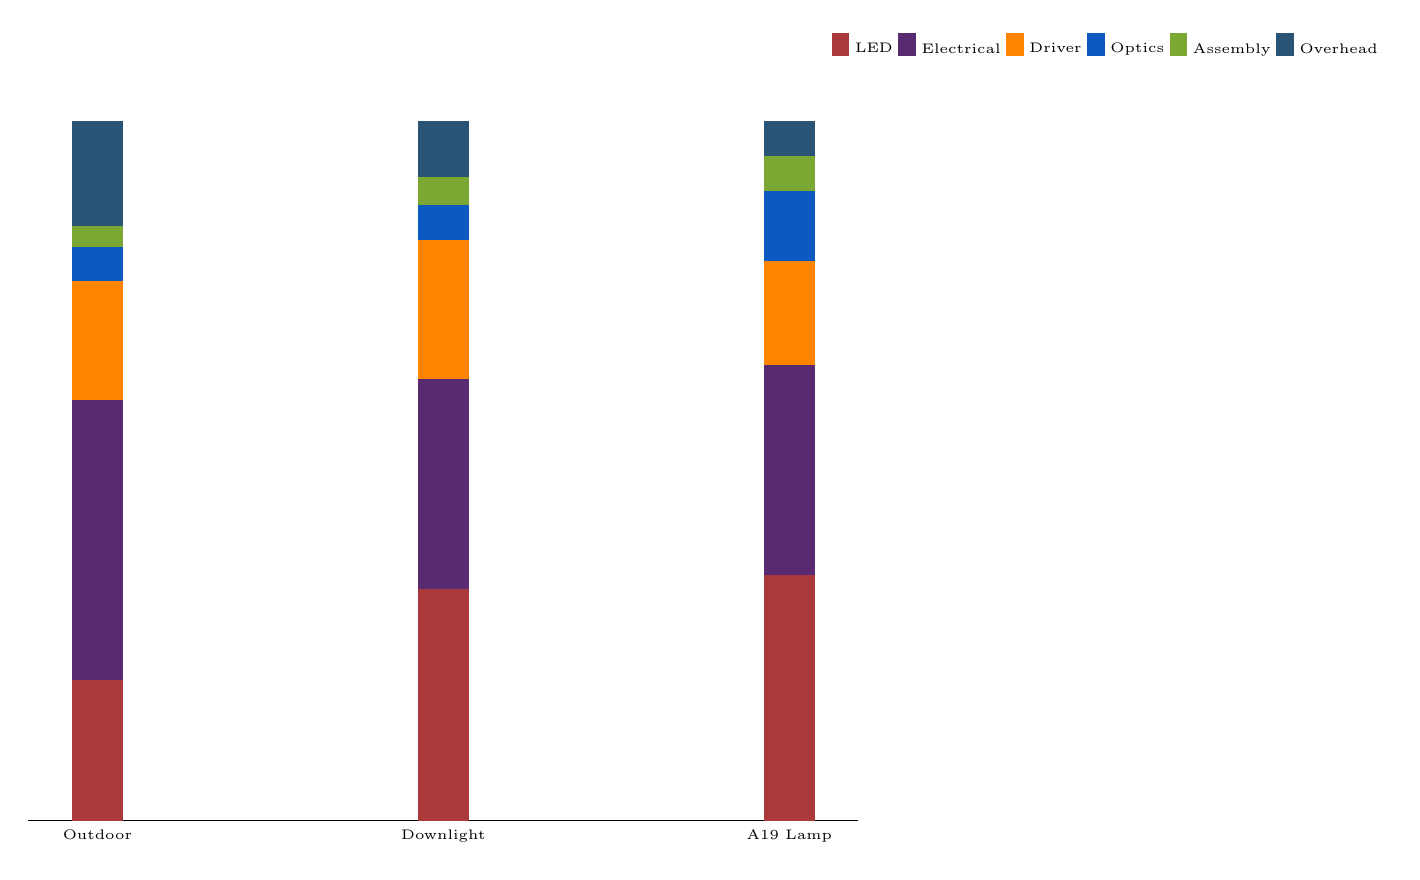
\begin{tikzpicture}
        \begin{axis}[
            width=\textwidth,
            ybar stacked,
        	bar width=18pt,
           % nodes near coords,
        	axis y line=none,
            axis x line*=bottom,
            ymin=0,
            ymax=100,
            symbolic x coords={
                Outdoor,
                Downlight,
                A19 Lamp},
            xtick=data,
            x tick label style={rotate=0,anchor=north, font=\tiny},
            legend style={
                legend columns = 6,
                at={(1.3,1.075)},
                anchor=south,
                draw=none,
                font=\tiny,},
        ]
        \addplot+[LED,fill=LED] plot coordinates
        {(Outdoor,20) (Downlight,33) (A19 Lamp,35)};
        \addplot+[TEM,fill=TEM] plot coordinates
        {(Outdoor,40) (Downlight,30) (A19 Lamp,30)};
        \addplot+[DRV,fill=DRV] plot coordinates
        {(Outdoor,17) (Downlight,20) (A19 Lamp,15)};
        \addplot+[OPT,fill=OPT] plot coordinates
        {(Outdoor,5) (Downlight,5) (A19 Lamp,10)};
        \addplot+[ASB,fill=ASB] plot coordinates
        {(Outdoor,3) (Downlight,4) (A19 Lamp,5)};
        \addplot+[OVH,fill=OVH] coordinates
        {(Outdoor,15) (Downlight,8) (A19 Lamp,5)};

        \legend{LED, Electrical, Driver, Optics, Assembly, Overhead}
        %\legend{\strut never, \strut rarely, \strut sometimes, \strut often}
        \end{axis}
    \end{tikzpicture}
    %\includegraphics[width=\textwidth]{./0_intro/img/cost_breakdown.png}
    \caption{}
    \label{fig:cost_breakdown}
\end{subfigure}
\begin{subfigure}[t]{.45\textwidth}
   \raggedleft
   %\includegraphics[width=\textwidth]{./0_intro/img/cost_breakdown_forecast.png}
   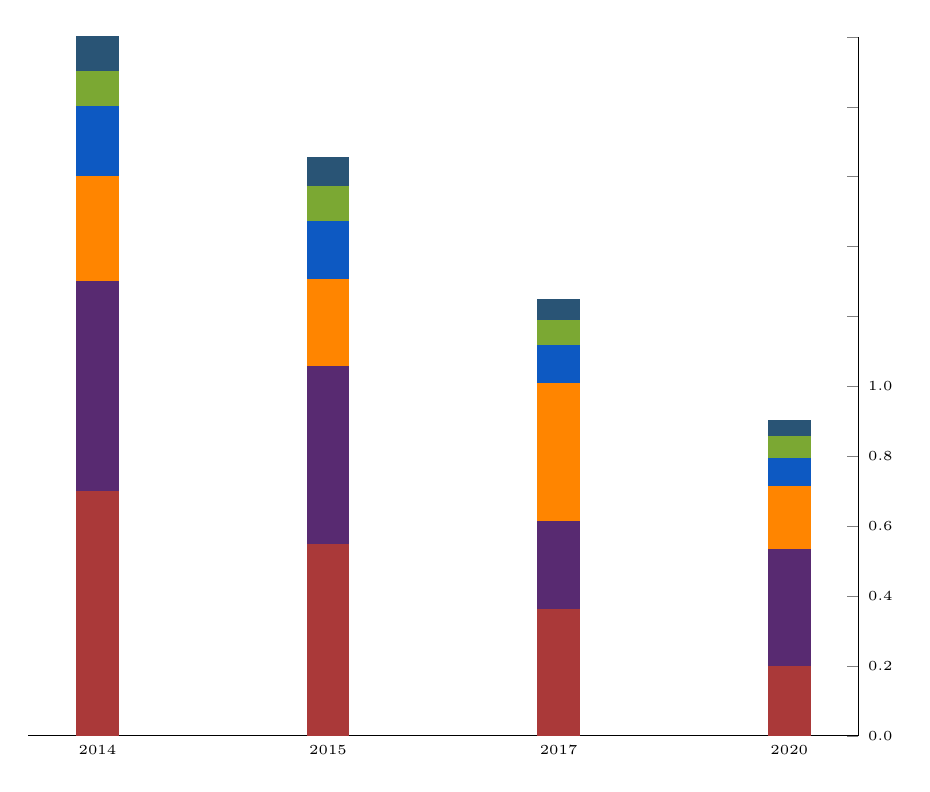
\begin{tikzpicture}
        \begin{axis}[
            width=\textwidth,
            ybar stacked,
        	bar width=15pt,
           % nodes near coords,
        	axis y line*=right,
            axis x line*=bottom,
            ymin=0,
            ymax=100,
            symbolic x coords={
                2014,
                2015,
                2017,
                2020},
            xtick=data,
            x tick label style={rotate=0,anchor=north, font=\tiny},
            y tick label style={rotate=0,anchor=west, font=\tiny},
            yticklabels={0,0.0, 0.2, 0.4, 0.6, 0.8,1.0},
        ]
        \addplot+[LED,fill=LED] plot coordinates
        {(2014,35) (2015,27.3) (2017,18) (2020,9.9)};
        \addplot+[TEM,fill=TEM] plot coordinates
        {(2014,30) (2015,25.6) (2017,12.6) (2020,16.7)};
        \addplot+[DRV,fill=DRV] plot coordinates
        {(2014,15) (2015,12.4) (2017,19.8) (2020,9)};
        \addplot+[OPT,fill=OPT] plot coordinates
        {(2014,10) (2015,8.3)  (2017,5.4) (2020,4.1)};
        \addplot+[ASB,fill=ASB] plot coordinates
        {(2014,5) (2015,5)     (2017,3.6) (2020,3.15)};
        \addplot+[OVH,fill=OVH] coordinates
        {(2014,5) (2015,4.1)   (2017,3) (2020,2.25)};



        \end{axis}
    \end{tikzpicture}
   \caption{}
   \label{fig:cost_breakdown_forecast}
\end{subfigure}
\caption{\emph{Left}-Comparison of cost breakdown for different lighting applications; \emph{right} - Cost breakdown projection for a typical A19 replacement lamp\\
\emph{Source: DOE SSL Roundtable and Workshop attendees}}
\label{fig:costs_BD_FC}
\end{figure}

%\begin{figure}[!h]
%    \centering
%    \includegraphics[width=.85\textwidth]{./0_intro/img/cost_breakdown.png}
%    \caption{Comparison of cost breakdown for different lighting applications\\
%            \emph{Source: DOE SSL Roundtable and Workshop attendees}}
%    \label{fig:cost_breakdown}
%\end{figure}
%
%\begin{figure}[!h]
%   \centering
%   \includegraphics[width=.85\textwidth]{./0_intro/img/cost_breakdown_forecast.png}
%   \caption{Cost breakdown projection for a typical A19 replacement lamp \\
%            \emph{Source: DOE SSL Roundtable and Workshop attendees}}
%   \label{fig:cost_breakdown_forecast}
%\end{figure}

LED or LED package \footnote{Electronic part composed by an assembly of LEDs connected in series or parallel and mounted in a single substrate} play their main role in the price of the lamp. Innovations are populating the market with three available technologies based in current capability of the chip: low, mid and high power range. The different offer in chip packages brings more flexibility at the system level in terms of optical design, luminarie light projection, color and driver design. Helping to provide solutions for all the different required applications. However full potential of the reduced profile of the LED has not yet been explored in regard to the luminaire design. Further research at the die level will improve the reliability of manufacturing process and the efficiency reducing the costs of the lamps, but is in the better use of the small size of the LED what will provide more value for the future lamp designs.

\begin{figure}[!h]
    \centering
    \includegraphics[width=8cm]{./0_intro/img/exploded_bulb_2.jpg}
    \caption{Exploded vision of an LED light bulb.}
    \label{fig:exploded_bulb}
\end{figure}


The Mechanical/Thermal/Electrical group - comprises heat sink, socket connector, PCBs and \emph{Electromagnetic Interference} (EMI) filters - still plays a dominant role in the design of the lamp. The heat sink and the connector are in many cases the body of the lamp where the heat sink and assembles the entire lamp. Traditional sockets, which are not design friendly, are currently kept in order to provide a fast transition for the current first wave of the \emph{LEDification}, the replacement period. Replacement lamps are also known as \emph{retrofit}\footnote{Adding the new LED technology to the older light bulb systems. In that way the end user can directly replace an incandescent lamp or a florescent tub by an LED one without needing to make any change in the current installation.} lamps. The current offer of \emph{retrofitted} LED bulbs is already an evident prove of the successes achieved in that area, nowadays is already possible to find a replacement lamp for almost all sorts of old lamps. However \emph{retrofited} lamps will have an small market share as predicted in the lighting forecast of Figure~\ref{fig:lighting_forecast}. That is why innovations in the Mechanical/Thermal/Electrical group will be necessary for the coming light fixtures, to evolve and reinvent the future LED luminaries, where the small size, the low profile and the colored lights of the LEDs will play an relevant role.


The driver is, with no doubt, the most \emph{special} component of the entire lamp. It is referred as \emph{special} because it is the only element of the lamp that plays a role in the three factors of influence for market penetration: Intelligence, Design and Costs. First, the driver is the only element that brings active functionality to the lamp, hence the only one that can incorporate the control and interactivity to the system. Second, its volume and its location influences the design of the lamp, the closer the driver to the LEDs is, the better the controllability and the intelligence of the system becomes. Finally the costs, what up-to-now have been the main research motivation for LED drivers.

Cost down reduction has enabled to bring the prices for simple \emph{retrofited} lamps down to competitive levels for the last years. However the chosen circuit architectures for low cost drivers are very cost sensitive towards more intelligent drivers, as it can be seen with the different prices for the \emph{dimmable}, \emph{non-dimmable} and \emph{smart} lamps of  Table~\ref{tab:lighting_tech}. That is why, a different approach in the driver architectures must be taken in order to respond the challenges for the future intelligent and connected LED lamps. In other words, the driver architecture that will provide power management, intelligence and connectivity together assembled in a reduced volume and at low cost will be, with no discussion, the key element to vertebrate the future of LED lighting technology.

The current driver architectures are based in discrete implementations. In such approach driver circuits are composed by different discrete components all assembled in a single \emph{printed-circuit-board}, what enables a fast development and cheap driver, because many of the mounted parts are general propose components sold by millions; however this approach has different limitations. First the performance of old and cheap components limit the volume reduction of the required  passive components in the drivers filters and magnetics. Second, as the circuit increases in complexity the \emph{bill of materials} (BOM) increases, also the costs, therefore reducing the possibilities to offer more functionalities in the driver circuit, such us connectivity and controllability at reduced costs. In resume, fulfill the driver requirements for the second generation of LED lamps will be very challenging using  discrete driver  architectures.

The approach to meet the requirements for the future lamps will probably relay in an integrated driver solution; meaning by integrated an \emph{application-specific integrated circuit} or ASIC. This approach brings the focus of the research in drivers  from the perspective of the integrated power supplies, where the power converter can be partially or fully integrated in a single package. There are two approaches of integrated power converters: \emph{Power System on Chip} (PSoC) or  \emph{Power System in Package} (PSiP). The first integrate all required power components, active and passive, in a single die. The second assemble all the components within the same package, keeping the appearance of an unique \emph{Integrated Circuit} (IC), see Figure~\ref{fig:psoc_example}. The advantages of having an integrated power management unit align with the necessities of the LED drivers, therefore trend of the drivers will be going towards having \emph{Power LED Drivers in Package} (PLDiP).

\begin{figure}[!h]
    \centering
    \includegraphics[width=6cm]{./0_intro/img/FSolzbacher01.jpg}
    \caption{Power System in a Package buck converter.}
    \label{fig:psoc_example}
\end{figure}

Besides the size reduction that an integrated driver would suppose, such approach would also bring other benefits in terms of control and connectivity.  The power management unit and driver control unit could possibly be integrated together, providing the necessary intelligence for light control and the connectivity optimized for the requirements of the coming connected lighting industry. The Philips \emph{HUE} lamp is a clear example of the requirements of the so called \emph{smart drivers}. The \emph{HUE} lamp is wireless connected to a network providing remote control through for the light intensity level and color from the a web interface, a mobile application or a dedicated remote control. The internal electronics has four LED drivers - on per color channel red, green, blue and amber - and, at the same time, ZigBee wireless interface, being the electronic board populated with discrete power drivers and micro-controller units. A solution capable to integrates all the functions in a single IC, or few ICs (one per channel), will definitely reduce packaging and assembling costs and still providing the same functionalities. At the same time, the expected market volume for SSL technologies will, with no doubt,  justify costs of a dedicated ASIC design for LED drivers. All-in-all has been the motivation of this PhD thesis with  the goal to explore and identify new architectures suitable for  integration that can efficiently power LEDs.



\section{Why a LED needs a driver?}

As shown in Figure~\ref{fig:led_I-V} a LED has a very abrupt \emph{voltage-current} ($v-i$) curve. For voltages below the \emph{forward voltage}, $v_{f}$, there is no current flow and the LED behaves as an open circuit. For voltages above $v_{f}$ the curve becomes very steep and the current increases dramatically with respect to the voltage, thus the LED behaves as a short circuit. Therefore the LED to be supplied at an specific point $P$  in order to provide the desired light output as shown in Figure~\ref{fig:led_I-V}, and depending on the position light colour and intensity will vary. Due to the steepness in the $v-i$ curve, the practical way to bias a LED is supplying them by current. Since the common used energy sources are voltage supplies, it is necessary a circuit that converts the input energy form the voltage source to a constat current for the LED, and that circuit is indeed the LED driver.

\begin{figure}[!h]
\centering

\begin{tikzpicture}[domain=0:6]
    \draw [->] (0,0) -- (5.5,0) node[anchor=west]{$v$};
    \draw [->] (0,0) -- (0,5.5) node[anchor=east]{$i$};

    %Mark Vth
    \draw (2,2pt) -- (2,-5pt) node[anchor=north] {$v_{f}$};

    %Mark Vthmin and Vt_max
    \def\dvf{0.25}
    \def\dvftop{0.45}

    \draw (1.5,2pt) -- (1.5,-5pt) node[anchor=north] {};
    \draw (2.5,2pt) -- (2.5,-5pt) node[anchor=north] {};
    \draw[dotted] (1.5,0) -- (1.5,\dvftop);
    \draw[dotted] (2.5,0) -- (2.5,\dvftop);
    %Mark Delta Vf
    \draw[pil,>-< ,dotted] (1.25,\dvf) -- (2.75,\dvf);
    \draw (1,\dvf) -- (1.5,\dvf) node[anchor=south east] {$\Delta v_f$};


    %Draw ideal plot
    \draw[thick] (0,0) -- (2,0) -- (4.5,5);

    %Draw lower limit
    \draw[dashed] (0,0) -- (1.5,0) -- (4,5);
    %Draw higher limit
    \draw[dashed] (0,0) -- (2.5,0) -- (5,5);

    %Draw bias point projection
    \draw[dotted] (4,4) -- (4,-0);
    \draw (4,2pt) -- (4,-5pt) node[anchor=north]  {$v_{bias}$};

    \draw[dotted] (4,4) -- (-0,4);
    \draw (2pt,4) -- (-5pt,4) node[anchor=east]  {$i_{bias}$};

    %Draw bias point
    \filldraw (4,4) circle(2pt) node[anchor=south west] {$P$};

    %Draw bias point variations
    \draw (4.5,4)  node[anchor=south west] {};
    \draw (3.5,4)  node[anchor=south west] {};

    %\draw[loosely dotted] (4.5,4) -- (4.5,-0);
    %\draw[loosely dotted] (3.5,4) -- (3.5,-0);
    \draw (4,2pt) -- (4,-5pt) node[anchor=north]  {$v_{bias}$};
    %Mark Vthmin and Vt_max
    \def\bpmi{4.5}
    \def\bpMa{3.5}
    %\draw (1.5,2pt) -- (1.5,-5pt) node[anchor=north] {};
    %\draw (2.5,2pt) -- (2.5,-5pt) node[anchor=north] {};
    %\draw[dotted] (1.5,0) -- (1.5,\dvftop);
    %\draw[dotted] (2.5,0) -- (2.5,\dvftop);
    %Mark Delta Vf
    %\draw[pil,>-< ,dotted] (3.25,\dvf) -- (4.75,\dvf);
    %\draw (4.5,\dvf) -- (5,\dvf) node[anchor=south west] {$\Delta V_{bias}$};

    %Mark Vthmin and Vt_max
    \def\dvf{4}
    %\draw (1.5,2pt) -- (1.5,-5pt) node[anchor=north] {};
    %\draw (2.5,2pt) -- (2.5,-5pt) node[anchor=north] {};
    %\draw[dotted] (1.5,0) -- (1.5,\dvftop);
    %\draw[dotted] (2.5,0) -- (2.5,\dvftop);
    %Mark Delta Vf
    \draw[pil,>-< ,dotted] (3.25,\dvf) -- (4.75,\dvf);
    \draw (4.5,\dvf) -- (5,\dvf) node[anchor=south west] {$\Delta v_{bias}$};


\end{tikzpicture}
\caption{Idealized LED voltage-current with the \emph{forward voltage} $v_f$  identified and projection of  the \emph{bias point} P }
\label{fig:led_I-V}
\end{figure}

At the first glance, keeping a constant bias current, $i_bias$, through the LED does not seems to be challenging. However LED V-I characteristic is not static, in practice LEDs have different sources of deviations and the LED drivers have to deal with them in order to keep delivering the desired light output. First, $V_f$ has a negative dependence with the temperature, drooping its values as the PN junction temperature increases. Second, the LED has an aging factor which derates the light output over time, and has to be adjusted by changing the bias point. And last, during production LEDs will vary in colour, flux and forward voltage; even for products from the same batch. The manufacturers have reduced the dispersion between devices by binning \footnote{Quality control performed at LED production line, where each LED is individual tested and sorted in groups (bins) that have the same electrical and lighting characteristics.}, but still after binning, the parts suffer deviations, \emph{e.g.} $10\%$ in $V_f$. Figure ~\ref{fig:led_I-V} shows graphicly how deviations in $V_f$ produce a displacement in the V-I characteristic,  which require to modify the $V_{bias}$ within a certain range $\Delta V_{bias}$ in order to keep $I_{bias}$ constant. All-in-all LEDs lamps have to
provide certain desired light output (or range) despite variations in the LED characteristics or of the voltage supply, thus is that control function which adds special complexity to the driver circuit.


There are three families of LED drivers that will be presented in the following sections from the integrate power supplies perspective.

\section{Linear Drivers}

Linear drivers place a shunt element between the source and the load(\emph{i.e} the LED). The shunt element limits the LED current providing the necessary voltage droop between the source and the load. The excess of voltage between the source and the load is dissipated in the shunt element, literally burned in form of heat; therefore these drivers become very inefficient if the LED voltage is not close to the source. Other limitation is that linear drivers only provide step-down conversion, thus they cannot work when the voltage at the load is higher than the input supply.

\begin{figure}[!h]
\centering
\ctikzset { bipoles/length=1cm}
\begin{subfigure}[t]{.45\textwidth}
    \centering
    \begin{circuitikz} [scale=0.65]
    \draw
        (5,0) to[short]
        (0,0) to[V = $v_{src}$]
        (0,3) to[generic=${Shunt}$,i=$i_o$]
        (5,3);
    \draw (5,0) to[leD*,v_>=$v_{o}$] (5,3);
    \end{circuitikz}
    \caption{}
    \label{fig:linear_ckt}
\end{subfigure}
\begin{subfigure}[t]{.45\textwidth}
    \begin{circuitikz} [scale=0.65]
    \begin{scope}%[xshift = 8cm, yshift=0cm]
        \draw[->] (0,0) -- (4,0) node[anchor=south] {$  m $};
        \draw[->] (0,0) -- (0,3.2) node[anchor=east] {$\eta $};

        %Ticks X
        \draw (3,-5pt) -- (3,2pt)  node[anchor=south west] {$1$};
        \draw (1.5,-5pt) -- (1.5,2pt)   node[anchor=south west] {$0.7$};

        %Ticks Y
        \draw (2pt,2.5) -- (-5pt,2.5) node[anchor=east] {$100\%$};
        \draw (2pt,1.5) -- (-5pt,1.5) node[anchor=east] {$70\%$};

        %Markers
        \draw[dotted] (3,2.5) -- (3,0);
        \draw[dotted] (3,2.5) -- (0,2.5);
        \draw[dotted] (1.5,1.5) -- (1.5,0);
        \draw[dotted] (1.5,1.5) -- (0,1.5);


        \draw[thick] (3,2.5) -- (0,0.5);
    \end{scope}
    \end{circuitikz}
    \caption{}
\label{fig:linear_chr}
\end{subfigure}
\caption{Linear driver, \emph{left}- schematic; \emph{righ}- conversion ratio vs. efficiency characteristics}
\label{fig:linear_drv}
\end{figure}

The circuit of the Figure~\ref{fig:linear_ckt} shows schematic of a linear driver, the shunt element can be implemented with just a resistor of with an active device. The firs will impose a current depending on the input source and the load conditions; the second will provide regulation of the bias point for variations in the source and in the load. Linear drivers are very simple to implement, with very low costs and taking almost no volume, being indeed the perfect solution for integration.


The plotted graph in Figure~\ref{fig:linear_chr} presents the variation of the driver efficiency with respect to the conversion ration $m$. Where $m$  is the ratio between the input voltage, $v_{src}$,  and the output voltage,$v_o$, being defined as
   \begin{equation}
        m = \frac{v_o}{v_{src}}.
   \end{equation}

The efficiency of the driver is the ratio between the input power and the output power
   \begin{equation}
        \eta = \frac{P_o}{P_i} = \frac{v_o i_o}{v_{src} i_o} = \frac{v_o}{v_{src}},
   \end{equation}

hence for this case the efficiency is indeed equal to the conversion ratio
   \begin{equation}
        \eta = m,
   \end{equation}
owing to the fact that LED drivers have to be efficient, saying that at worst case 80\% efficiency can be accepted, such drivers could only be suitable where the ration between input voltage and load voltage is 0.8.

Despite the fact that linear drivers are cheap and easy to integrate, their poor efficiencies  palace them in a unfavorable position for a suitable architecture for an integrated solution.

\section{Inductor Based Converters}

\emph{Inductor Based Converters} (IBCs) are \emph{Switched Mode Power Supplies} (SMPS) \footnote{Electronic power supply that provides efficient electric power conversion by commuting between different circuit configurations (modes).}  that employ magnetic passive elements (i.e. inductors and transformers) to store energy and provide efficient electrical power conversion. Since IBCs have are very efficient in voltage-to-current conversion they are ideal as LED drivers.

These converters can provide step-up and step-down conversion for large dynamic ranges while keeping the efficiency very high. On top of their power conversion capabilities, such converters can also provide galvanic isolation, which in many applications, is compulsory in order to guarantee the safety of the users against electrical hazards. Such characteristics place these drivers as the preferred solution for the LED industry. Figure~\ref{fig:induct_ckt} shows one of the most popular implementations for LED drivers the \emph{buck} converter.  Figure~\ref{fig:induc_chr} presents the regulation characteristic curve of a generic  inductor based converter. As shown, the theoretical efficiency of these converters is 100\% for all the conversion ratio range, in practice due to parasitics in switches and inductors, the efficiency drops to a certain value with small fluctuations with respect to the conversion range.

\begin{figure}[!h]
\centering
\ctikzset { bipoles/length=1cm}
\begin{subfigure}[t]{.45\textwidth}
    %\centering
    \raggedright
    \begin{circuitikz} [scale=0.65]
    \draw
        (6.5,0) to[short]
        (0,0) to[V = $v_{src}$]
        (0,3) to[switch]
        (3,3) to[inductor=${L}$,i=$i_o$]
        (6.5,3);

    \draw (2.5,3) to[switch] (2.5,0);

    \draw (6.5,0) to[leD*,v_>=$v_{o}$] (6.5,3);

    \end{circuitikz}
    \caption{}
    \label{fig:induct_ckt}
\end{subfigure}
\begin{subfigure}[t]{.45\textwidth}
    %\centering
    \raggedleft
    \begin{circuitikz} [scale=0.65]
    \begin{scope}%[xshift = 8cm, yshift=0cm]
        \draw[->] (0,0) -- (4,0) node[anchor=south] {$  m $};
        \draw[->] (0,0) -- (0,3.2) node[anchor=east] {$\eta $};

        %Ticks X
        %\draw (3,2pt) -- (3,-5pt) node[anchor=north] {$1$};
        %\draw (1.5,2pt) -- (1.5,-5pt) node[anchor=north] {$0.7$};

        %Ticks Y
        \draw (2pt,2.5) -- (-5pt,2.5) node[anchor=east] {$100\%$};
        \draw (2pt,1.5) -- (-5pt,1.5) node[anchor=east] {$90\%$};

        %Markers
        % \draw[dotted] (3,2.5) -- (3,0);
        \draw[dotted] (3,2.5) -- (0,2.5);
        %\draw[dotted] (1.5,1.5) -- (1.5,0);
        \draw[dotted] (1.5,1.5) -- (0,1.5);


        \draw[thick] (0.5,2.5) -- (3,2.5) node[anchor=south] {$Theoretical$};
        \draw[thick,dashed] (0.5,1.20) parabola[bend at end] (3,1.7) node[anchor=north] {$Real$};
    \end{scope}
    \end{circuitikz}
    \caption{}
\label{fig:induc_chr}
\end{subfigure}
\caption{Inductor based converter, \emph{left} - buck converter schematic; \emph{right} - conversion ration \emph{vs.} efficiency curve comparing the \emph{theoretical} and a \emph{practical} limit. }
\label{fig:inductive_smps}
\end{figure}

On of the disadvantage of these converters are the magnetics, and the volume related to them. In practice, inductors dominate the entire volume of the LED drivers as shown in Figure~\ref{fig:smps_driver}. Integrated implementations of these converters suffer the challenges of using integrated magnetic components. The present \emph{very-large integration scale} (VLSI) technologies do not yet offer power inductors in the commercial implementations, and other integrated inductors are not yet mature for products out of the research phase.

Yet another disadvantage for integration is the voltage stress in the switches of the converter. Switches in inductive converters have to withstand the full operational voltage, which depending on the application range from tens to few hundred of volts. Using high voltage devices have three main drawbacks: First, the losses in the devices scale quadratically with the voltage  stress. Second, worst switching performances, being high voltage devices less efficient and slower in the switching transitions. Third, the standard VLSI technologies do not offer these devices and the VLSI technologies that offer them are less performance and more expensive than the dedicated discrete technologies.

\begin{figure}[!h]
\centering
\begin{tikzpicture}
\node[anchor=south west,inner sep=0] (image) at (0,0) {\includegraphics[height=5cm,angle=90]{./0_intro/img/LED_driver.png}};
\begin{scope}[x={(image.south east)},y={(image.north west)}]
%\draw [<-,thick] (0.75,0.5) -- (0.855,0.7)  node [anchor=south west] {Power Magnet};
\draw[red,ultra thick,rounded corners] (0.70,0.3805) rectangle (0.855,0.7);
\draw[red,ultra thick,rounded corners] (0.11,0.1) rectangle (0.28,0.50);
\draw[red,ultra thick,rounded corners] (0.28,0.1) rectangle (0.63,0.62);
\end{scope}
\end{tikzpicture}
\caption{Magnetic components marked with a red square in a mains connected LED driver. The magnetic components dominate the volume of the converter.}
\label{fig:smps_driver}
\end{figure}


\section{Switched Capacitors}
Switched Capacitor Converters (SCCs) are SMPS composed only by switches and capacitors that provide efficient voltage conversion. SCC where initially used for voltage multiplication and more recently in applications that need voltage regulation as well. Compared to inductor based converters, the absence of magnetic elements places them in a better position for high density power systems and integrated solutions, such as Power-System-in-Package (PSiP) or Power-System-on-Chip (PSoC).

SCCs have a fix ratio of conversion between the input and the output determined by the topology. The output voltage of the converter under no load conditions is defined as \emph{target voltage} $v_t$. The converter performs at high efficiency when the load is supplied close to the \emph{target voltage}. Similar to the linear drivers, if the output voltage goes below the \emph{target voltage} the efficiency drops and when the output voltage is above their \emph{target voltage} the converter cannot operate. Figure~\ref{fig:SCC_ckt} shows a step-down converter with a conversion ratio of one half.

A common practice to extend the regulation margins of these converters is to have topologies with multiple conversion rations. From Figure~\ref{fig:SCC_chr} it can be seen that the efficiency increases as the ration $m$ gets close to the first fixed conversion ration of the converter $m_1$; right after $m_1$ the efficiency drops again dramatically and it again linearly increases as it approaches the second fixed conversion ratio of the converter $m_2$. Beyond $m_2$ the converter does not work.


\begin{figure}[!h]
\centering
\ctikzset { bipoles/length=1cm}
\begin{subfigure}[t]{.45\textwidth}
    %\centering
    \raggedright
    \begin{circuitikz} [scale=0.65]
    \draw
        (6.5,0) to[short]
        (0,0) to[V = $v_{src}$]
        (0,3) to[switch]
        (2,3) to[capacitor=${C_1}$]
        (3,3) to[switch]
        (5,3) to[short]
        (6.5,3);

    %Parallel switch to ground
    \draw (3.25,3) to[switch] (3.25,0);

    %Switch branch to load
    \draw (1.75,3) --
          (1.75,4.5) to[switch]
          (5,4.5) --
          (5,3);

    %Load and capacitor C2
    \draw (5,0) to[capacitor=$C_2$] (5,3);
    \draw (6.5,0) to[leD*,v_>=$v_{o}$] (6.5,3);

    \end{circuitikz}
    \caption{}
    \label{fig:SCC_ckt}
\end{subfigure}
\begin{subfigure}[t]{.45\textwidth}
    %\centering
    \raggedleft
    \begin{circuitikz} [scale=0.65]
    \begin{scope}[xshift = 10cm, yshift=0cm]
            \draw[->] (0,0) -- (4,0) node[anchor=south west] {$  m $};
            \draw[->] (0,0) -- (0,3.2) node[anchor=east] {$\eta $};

            %Ticks X
            \draw  (1.75,5pt) -- (1.75,0pt) node[anchor=south west ] {$m_1$};
            \draw  (3,5pt) -- (3,0pt)   node[anchor=south west ] {$m_2$};
            %\draw (1.5,2pt) -- (1.5,-5pt) node[anchor=north] {$0.7$};

            %Ticks Y
            \draw (2pt,2.5) -- (-5pt,2.5) node[anchor=east] {$100\%$};
            \draw (2pt,1.5) -- (-5pt,1.5) node[anchor=east] {$90\%$};

            %Markers
            \draw[dotted] (1.75,2.4) -- (1.75,0);
            \draw[dotted] (3,2.3) -- (3,0);
            \draw[dotted] (3,2.5) -- (0,2.5);
            %\draw[dotted] (1.5,1.5) -- (1.5,0);
            %\draw[dotted] (1.5,1.5) -- (0,1.5);


            \draw[thick] (0.5,1.4) -- (1.75,2.4) -- (1.75,1.6) -- (3,2.3)  node[anchor=south] {};
            %\draw[thick,dashed] (0.5,1.20) parabola[bend at end] (3,1.7)[anchor=north] {};
        \end{scope}
    \end{circuitikz}
    \caption{}
\label{fig:SCC_chr}
\end{subfigure}
\caption{Switched capacitor converter, \emph{left} - 2:1 converter schematic; \emph{right} - conversion ration \emph{vs.} efficiency curve for of a generic multiple  conversion ration stage }
\label{fig:SCC_smps}
\end{figure}

The main advantages of these converters is that they use no inductors, which make them very favorable for integration. Integrated capacitors have a better energy density than integrated inductors. The mechanical structure of the capacitors, a stack of isolator-metal-isolator, is much easier to replicate in small scale. Yet another advantage of the switch capacitors is that they split the voltage applied to the converter among the different components, thus reducing the voltage stress in the switches and capacitors. Such voltage stress reduction is very interesting from the point of view of integration. First, lower voltage capacitors have better performances: more energy density, less derating and better chances of integration. Second, lower voltage switches have better switching performances. Finally, low voltage devices take less silicon area and there is more offer in the standard VLSI technologies, thus reducing the production costs.

The big disadvantage of these converters is that they can not directly provide the voltage-to-current conversion required for the LEDs to work. Nevertheless they are still used as LED drivers in backlighting applications in battery supplied devices. In such cases, the SCCs steps-up or steps-down the battery voltage and afterwards a linear driver  provides current regulation to bias properly the LEDs. Adopting that architecture for general lighting could be a solution but when  voltages and currents are scaled to the values used in these applications the number of necessary conversion steps of the SCC would make it totally infeasible and inefficient.

Based on the previous arguments could lead that adopting an SCC architecture for as a general solution for LED drivers seems to be , a priory,  not an evident choice. On the one hand, their limitation in voltage-to-current conversion would place switched capacitors directly out of the possible candidates. However, on the other hand, the advantageous characteristics of switched capacitors for integration made this circuits very attractive. Actually if the initial limitations in voltage-to-current conversion could be overcame, such architecture would be an interesting candidate to explore as a solution for a Power System \emph{on-Chip/in-Package} LED driver. Therefore the last statement was the research motivation  of this PhD dissertation.


This book is divided in the four main sections that where necessary to build a switched capacitor LED driver. The first section introduces the new LED driver architecture used during the entire thesis, the \emph{Hybrid-Switched Capacitor Converter}, H-SCC from now on. The second part of this book, the core of the PhD. work, presents the methodology to model H-SCC. The methodology extends the previous works in the topic providing an enhanced modeling for the design of SCCs and H-SCCs. The third section is devoted to the practical use of the new methodology, thus for the design phase of a converter. The modeling is used  to help in the development facilitating the sizing and optimization of the design variables. The last section presents a discrete implementation of 12W H-SCC LED driver and the design procedure. Although is not a regular practice, experimental work is not only presented in the in the last section. The experimental work has been also  used to validate the presented modeling and methodology. The final section is the conclusion of the entire work and the future opportunities that the presented work can offer.
